\chapter{Architektura i działanie systemu}\label{ch:architektura-i-dzialanie}

Niniejszy rozdział przedstawia koncepcję architektoniczną opracowanego systemu, sposób integracji poszczególnych komponentów oraz szczegółową charakterystykę działania czterech modułów funkcjonalnych wraz z opisem algorytmów w postaci pseudokodu.

\section{Architektura ogólna i integracja modułów}\label{sec:architektura-narzedzia}

\subsection{Struktura modułowa i tryby pracy narzędzia}\label{subsec:struktura-modulowa-cli}

Opracowane rozwiązanie składa się z komponentu klienckiego uruchamianego na stacji roboczej Windows (główny skrypt \file{firewall.ps1} wdrażany w katalogu produkcyjnym jako \file{C:\FW\FirewallRules.ps1} wraz z dołączanymi modułami kopii zapasowych \file{backup\Backup-Create.ps1} i \file{backup\Backup-Restore.ps1}) oraz komponentu serwerowego działającego na maszynie z systemem Ubuntu Linux (\file{/usr/local/bin/fw-server.sh} wraz z usługą SFTPGo).

Główny skrypt systemu może być wywoływany w trzech rozłącznych trybach operacyjnych:
\begin{enumerate}
    \item \textbf{Tryb interaktywny CLI (domyślny)} - przeznaczony dla administratora pracującego w oknie konsoli z podniesionymi uprawnieniami. Przy starcie automatycznie wykonuje synchronizację stanu polityki zapory z bazą referencyjną audytu (\code{startup sync}), weryfikuje ochronę katalogu modułów kopii zapasowych, a następnie wyświetla dziesięciopunktowe menu główne wraz z dynamicznym paskiem statusu usługi \textit{Watcher} i bieżącej polityki awarii.
    \item \textbf{Tryb nieinteraktywnej synchronizacji audytu (\code{-SyncAudit})} - wywoływany w tle przez zadanie harmonogramu systemowego \code{\FirewallAudit\Watcher} działające na koncie \code{NT AUTHORITY\SYSTEM}. Skrypt oczekuje na ustabilizowanie serii zdarzeń w dzienniku zapory, porównuje cały magazyn rejestru oraz zasad grupy GPO z plikiem \file{baseline.json}, dopisuje wykryte zmiany zewnętrzne do dziennika \file{audit.jsonl}, aktualizuje plik stanu \file{state.json} i kończy pracę z kodem wyjścia \code{0}.
    \item \textbf{Tryb agenta eksportu kopii zapasowej (\code{-Agent Export})} - wywoływany zdalnie przez serwer kopii zapasowych za pośrednictwem wymuszonego polecenia SSH. W trybie tym standardowe wyjście procesu pełni rolę kanału protokołu komunikacyjnego: agent upewnia się, że reguła zezwalająca na ruch SSH z serwera kopii istnieje, eksportuje politykę zapory do pliku tymczasowego, oblicza jej skrót SHA-256 i przesyła dane zakodowane w formacie Base64 pomiędzy znacznikami \code{FWAGENT-BEGIN} oraz \code{FWAGENT-END}.
\end{enumerate}

Zestawienie wszystkich opcji interaktywnego menu głównego oraz odpowiadających im modułów funkcjonalnych przedstawiono w tabeli \ref{tab:menu-glowne}.

\begin{table}[H]
    \centering
    \caption{Struktura interaktywnego menu głównego systemu i przypisanie do modułów}\label{tab:menu-glowne}
    \tablefont
    \begin{tabularx}{\linewidth}{C{1.4cm} L{4.8cm} C{2.2cm} Y}
        \toprule
        \hcell{Opcja} & \hcell{Nazwa pozycji w menu} & \hcell{Moduł} & \hcell{Wykonywana operacja systemowa} \\
        \midrule
        \code{1} & \textit{Add Inbound Rule} & Moduły 1, 2 & Kreator reguły przychodzącej z walidacją IP/portu, wyborem protokołu i profilu, kopią \code{auto-add} oraz zapisem przez audyt. \\
        \code{2} & \textit{Add Outbound Rule} & Moduły 1, 2 & Kreator reguły wychodzącej z mapowaniem portu zdalnego, wyborem profilu, kopią \code{auto-add} i zapisem przez audyt. \\
        \code{3} & \textit{List Firewall Rules} & Moduły 1, 2 & Wyświetlenie aktywnego profilu połączenia NLA oraz tabeli reguł projektowych z prefiksem \code{OSO-}. \\
        \code{4} & \textit{Delete Firewall Rule} & Moduły 1, 2 & Wyświetlenie tabeli reguł i usunięcie wybranej pozycji po indeksie. \\
        \code{5} & \textit{View audit log} & Moduł 3 & Interaktywna przeglądarka dziennika \file{audit.jsonl} z filtrowaniem według liczby dni, typu operacji oraz źródła zmiany. \\
        \code{6} & \textit{Verify audit log integrity} & Moduł 3 & Pełna weryfikacja kryptograficznego łańcucha skrótów SHA-256, ciągłości numerów \code{seq} i opcjonalnego \textit{head hash}. \\
        \code{7} & \textit{Sync audit now} & Moduł 3 & Natychmiastowe porównanie bieżącej polityki w rejestrze z bazą \file{baseline.json} i rejestracja zmian zewnętrznych. \\
        \code{8} & \textit{Audit settings} & Moduł 3 & Podmenu zarządzania audytem: instalacja/usunięcie zadania \textit{Watcher} (\code{[I]}/\code{[U]}), przełącznik \textit{fail-closed}/\textit{fail-open} (\code{[F]}), odczyt \textit{head hash} (\code{[H]}). \\
        \code{9} & \textit{Backups} & Moduł 4 & Podmenu kopii zapasowych: ręczne utworzenie kopii na serwerze (\code{[B]}), lista kopii przez SFTP (\code{[L]}), przywracanie polityki (\code{[R]}). \\
        \code{10} & \textit{Exit} & Rdzeń CLI & Bezpieczne zakończenie pracy interaktywnej pętli programu. \\
        \bottomrule
    \end{tabularx}
\end{table}

\subsection{Wspólny kontrakt wykonania zmian polityki}\label{subsec:przeplyw-sterowania}

Kluczowym założeniem architektonicznym łączącym wszystkie cztery moduły jest zasada centralnej mediacji zmian. Żaden moduł funkcjonalny nie może samodzielnie wywołać polecenia modyfikującego stan zapory poza kontekstem transakcyjnego mechanizmu audytowego. W tym celu zdefiniowano jednolity kontrakt architektoniczny:
\begin{enumerate}
    \item Każda operacja zmieniająca politykę (dodanie reguły w Module 1, usunięcie reguły w Module 1, zmiana przypisania profili w Module 2, instalacja zadania \textit{Watcher} w Module 3 czy pełny import kopii zapasowej w Module 4) przekazuje właściwy blok wykonawczy do mechanizmu transakcyjnego wraz z deklaracją oczekiwanego zakresu modyfikacji:
    \begin{itemize}
        \item \code{NewRules} - akcja może wyłącznie utworzyć nowe reguły w magazynie (wykorzystywane przy dodawaniu reguł),
        \item \code{Names} - akcja może zmodyfikować lub usunąć wyłącznie reguły o jawnie przekazanych identyfikatorach systemowych (wykorzystywane przy usuwaniu i przełączaniu reguł),
        \item \code{Profiles} - akcja może zmienić wyłącznie globalne parametry profili \textit{Domain}, \textit{Private} lub \textit{Public},
        \item \code{All} - akcja obejmuje całą politykę zapory (wykorzystywane podczas odtwarzania pełnej kopii zapasowej \file{.wfw}).
    \end{itemize}
    \item Przed wywołaniem akcji dodania lub usunięcia reguły w interfejsie CLI wywoływany jest punkt kontrolny modułu kopii zapasowych (\code{pre-change backup}). Jeżeli serwer kopii jest nieosiągalny lub eksport zakończy się błędem, program wstrzymuje wykonanie i wymaga od administratora jawnej zgody na kontynuację bez kopii bezpieczeństwa (domyślnie operacja jest przerywana).
\end{enumerate}

\section{Moduł 1: Zarządzanie regułami zapory i walidacja parametrów}\label{sec:modul-reguly}

Pierwszy moduł funkcjonalny (autor: Adam Rola) odpowiada za interaktywne definiowanie, walidację, numerację, przeglądanie oraz usuwanie reguł filtrujących ruch sieciowy w kierunkach przychodzącym (\textit{Inbound}) i wychodzącym (\textit{Outbound}).

\subsection{Konwencja nazewnictwa i dynamiczna numeracja reguł}\label{subsec:schemat-prefiks-oso}

Aby rozwiązać problem przemieszania reguł tworzonych przez administratora z setkami wbudowanych reguł systemu Windows, wprowadzono ustrukturyzowaną konwencję nazewnictwa wyświetlanego:
\begin{equation}\label{eq:konwencja-nazewnictwa}
    \texttt{<NR>}\text{\texttt{-OSO-}}\texttt{<Action>}\text{\texttt{-}}\texttt{<Direction>}\text{\texttt{-}}\texttt{<HHmmss>}
\end{equation}
gdzie poszczególne elementy oznaczają:
\begin{itemize}
    \item \code{<NR>} - dwucyfrowy (lub wielocyfrowy dla wartości $\ge 100$) numer porządkowy formatowany z wiodącym zerem. Przed utworzeniem nowej reguły moduł przeszukuje wszystkie istniejące reguły zawierające wzorzec \code{OSO-}, wyodrębnia za pomocą wyrażenia regularnego \code{^(\d+)-OSO} najwyższy dotychczasowy numer $N_{\max}$ i nadaje nowej regule wartość $N_{\max} + 1$. Gwarantuje to brak kolizji numeracji nawet po wcześniejszym usunięciu środkowych reguł;
    \item \code{<Action>} - akcja filtru: \code{Allow} (zezwolenie) lub \code{Block} (blokada);
    \item \code{<Direction>} - kierunek przepływu pakietów: \code{Inbound} lub \code{Outbound};
    \item \code{<HHmmss>} - sześciocyfrowy znacznik czasu utworzenia reguły (godzina, minuta, sekunda), zapewniający pełną unikalność nazwy w obrębie sesji administracyjnej.
\end{itemize}

Przykładowa wygenerowana nazwa reguły blokującej ruch przychodzący ma postać \code{05-OSO-Block-Inbound-190556}. Warto przy tym wskazać na istotną różnicę pomiędzy nazwą wyświetlaną (\code{DisplayName}), w której osadzana jest powyższa sygnatura, a wewnętrznym identyfikatorem reguły (\code{Name}). W architekturze zapory Windows atrybut \code{Name} stanowi trwały klucz wartości w rejestrze (najczęściej generowany przez system unikalny GUID), natomiast moduł filtruje, sortuje i prezentuje reguły według atrybutu \code{DisplayName}.

\subsection{Walidacja danych wejściowych i semantyka kierunkowa portów}\label{subsec:walidacja-parametrow}

Kreator dodawania reguły prowadzi administratora przez kolejne parametry filtru, stosując wielostopniową walidację wejścia w pętlach kontrolnych:
\begin{enumerate}
    \item \textbf{Adres IP (\code{RemoteAddress})} - pole opcjonalne (naciśnięcie klawisza \code{Enter} oznacza dopasowanie do dowolnego adresu IP - \code{Any}). W przypadku podania wartości tekstowej jest ona weryfikowana za pomocą parsera klasy systemowej \code{[System.Net.IPAddress]::TryParse} z dodatkowym warunkiem obecności separatora kropkowego (\code{.}) dla IPv4 lub dwukropka (\code{:}) dla IPv6. Dodatkowy warunek eliminuje akceptację pojedynczych liczb całkowitych (np.\ \code{12345}), które standardowy parser .NET zinterpretowałby jako 32-bitowy zapis adresu IPv4.
    \item \textbf{Numer portu} - pole opcjonalne (pusty ciąg oznacza wszystkie porty - \code{Any}). Podana wartość musi przejść konwersję do typu całkowitego 32-bitowego oraz należeć do domkniętego przedziału poprawnych portów protokołów TCP/UDP.
    \item \textbf{Kierunkowe mapowanie portu (\code{LocalPort} vs \code{RemotePort})} - istotnym usprawnieniem względem ręcznej konfiguracji w GUI jest automatyczne przypisanie portu do właściwej strony połączenia w zależności od kierunku reguły:
    \begin{itemize}
        \item dla ruchu przychodzącego (\textit{Inbound}) podany numer portu jest bindowany jako \textbf{port lokalny} (\code{LocalPort}), ponieważ zapora chroni lokalnie nasłuchującą usługę (np.\ port 22 dla serwera SSH), do której klient zewnętrzny łączy się z losowego portu efemerycznego,
        \item dla ruchu wychodzącego (\textit{Outbound}) podany numer portu jest bindowany jako \textbf{port zdalny} (\code{RemotePort}), ponieważ celem reguły wychodzącej jest zablokowanie lub zezwolenie na komunikację z określoną usługą docelową na zdalnym hoście (np.\ port 53 dla zapytań DNS lub port 80/443 dla ruchu HTTP/HTTPS).
    \end{itemize}
    \item \textbf{Wymuszenie protokołu transportowego przy określonym porcie} - platforma WFP nie pozwala na zdefiniowanie filtru portowego bez wskazania protokołu warstwy transportowej (TCP lub UDP). Jeżeli administrator podał numer portu, selektor protokołu automatycznie blokuje opcję \code{Any} i ustawia protokół \code{TCP} jako domyślny wybór po naciśnięciu klawisza \code{Enter}. Jeżeli port nie został określony, domyślnym wyborem pozostaje dowolny protokół (\code{Any}).
\end{enumerate}

Przebieg interaktywnego tworzenia nowej reguły przychodzącej wraz z automatycznym wykonaniem kopii zapasowej i rejestracją w audycie przedstawiono na rysunku \ref{fig:menu-add-rule}.

\Figure[1.0]{menu_add_rule.png}{Widok głównego menu narzędzia oraz przebieg kreatora dodawania reguły przychodzącej z walidacją parametrów i automatyczną kopią zapasową}{fig:menu-add-rule}

\subsection{Przeglądanie, sortowanie i bezpieczne usuwanie reguł}\label{subsec:przegladanie-usuwanie-regul}

Opcje menu \code{3} (\textit{List Firewall Rules}) oraz \code{4} (\textit{Delete Firewall Rule}) pobierają z systemu wszystkie reguły posiadające w nazwie znacznik \code{OSO-}, a następnie wzbogacają każdy obiekt o powiązane filtry adresowe (\code{LocalAddress}, \code{RemoteAddress}) oraz portowe (\code{Protocol}, \code{LocalPort}, \code{RemotePort}).

Aby prezentowana tabela odzwierciedlała rzeczywistą kolejność ewaluacji reguł przez silnik zapory Windows, lista przed wyświetleniem jest sortowana dwupoziomowo:
\begin{enumerate}
    \item pierwszorzędnie malejąco według akcji (\code{Action}), dzięki czemu reguły blokujące (\code{Block}) są zawsze zgrupowane na górze tabeli przed regułami zezwalającymi (\code{Allow}),
    \item drugorzędnie rosnąco według nazwy wyświetlanej (\code{DisplayName}), czyli zgodnie z numerem porządkowym \code{<NR>-OSO}.
\end{enumerate}
Podczas usuwania reguły administrator nie musi przepisywać długiego identyfikatora GUID ani pełnej nazwy reguły - wybiera jedynie wiersz z tabeli za pomocą przypisanego indeksu liczbowego. Moduł weryfikuje poprawność indeksu, zleca utworzenie kopii zapasowej \code{auto-delete}, a następnie przekazuje unikalny identyfikator systemowy reguły (\code{Name}) oraz jej oczekiwaną nazwę wyświetlaną (\code{expectedDisplayName}) do transakcyjnego silnika audytu.

\section{Moduł 2: Kontekstowe zarządzanie profilami sieciowymi}\label{sec:modul-profile}

Drugi moduł funkcjonalny (autor: Aliaksei Lapachuk) odpowiada za integrację procesu zarządzania regułami z podsystemem rozpoznawania lokalizacji sieciowej NLA (\textit{Network Location Awareness}) oraz wieloprofilowym modelem bezpieczeństwa systemu Windows.

\subsection{Detekcja aktywnego profilu sieciowego i przypisywanie kontekstu}\label{subsec:detekcja-profilu}

Zanim administrator przystąpi do przeglądu lub usunięcia reguł (opcje menu \code{3} oraz \code{4}), moduł odpytuje podsystem sieciowy o aktualny stan wszystkich połączonych interfejsów (\cmd{Get-NetConnectionProfile}) i prezentuje zestawienie zawierające alias karty sieciowej (\code{InterfaceAlias}), nazwę zidentyfikowanej sieci (\code{Name}) oraz przypisaną przez usługę NLA kategorię bezpieczeństwa (\code{NetworkCategory}: \code{DomainAuthenticated}, \code{Private} lub \code{Public}). Pozwala to administratorowi natychmiast zweryfikować, który zestaw reguł profilowych jest w danej chwili egzekwowany przez jądro systemu na poszczególnych kartach sieciowych.

Podczas tworzenia każdej nowej reguły dedykowany selektor profili umożliwia przypisanie reguły do dowolnego podzbioru spośród trzech profili systemowych.

Administrator może wybrać pojedynczy profil (np.\ \code{3} dla sieci publicznej), podać listę profili rozdzielonych przecinkami lub spacjami (np.\ \code{2,3} dla jednoczesnego objęcia sieci prywatnych i publicznych, przy czym duplikaty są automatycznie usuwane) albo nacisnąć klawisz \code{Enter}, co przypisuje wartość \code{Any} (reguła aktywna niezależnie od lokalizacji sieciowej).

Widok wykrytego aktywnego profilu sieciowego (\code{Private} na interfejsie \code{Ethernet}) wraz z pełną tabelą skonfigurowanych reguł projektowych oraz przebiegiem usuwania reguły przedstawiono na rysunku \ref{fig:list-delete-rules}.

\Figure[1.0]{list_delete_rules.png}{Detekcja aktywnego profilu sieciowego (\code{Private}), tabela skonfigurowanych reguł \code{OSO-*} oraz procedura bezpiecznego usunięcia reguły po indeksie}{fig:list-delete-rules}

Formalny przebieg połączonego procesu walidacji parametrów, doboru protokołu i profili sieciowych, zabezpieczenia stanu na serwerze kopii oraz transakcyjnej rejestracji nowej reguły (Moduły 1 i 2) przedstawiono w algorytmie \ref{alg:tworzenie-reguly}.

\begin{algorithm}[H]
    \caption{Walidacja parametrów, dobór profilu sieciowego i rejestracja nowej reguły zapory}\label{alg:tworzenie-reguly}
    \Input{Wybrany kierunek ruchu $D \in \{\texttt{Inbound}, \texttt{Outbound}\}$, aktualny zbiór reguł systemowych $\mathcal{R}$}
    \Output{Status utworzenia nowej reguły zapory oraz rekordy transakcyjne w dzienniku audytu}
    $N_{\max} \leftarrow \max\bigl(\{0\} \cup \{k \in \NN \mid \exists r \in \mathcal{R}\colon \operatorname{DisplayName}(r) \text{ zaczyna się od } k\text{\texttt{-OSO}}\}\bigr)$;\;
    $\mathit{prefix} \leftarrow \operatorname{FormatTwoDigits}(N_{\max} + 1)$\;
    Wczytaj w pętli walidacyjnej adres IP $A$ ($\texttt{Any}$ dla pustego wejścia lub poprawny IPv4/IPv6 z separatorem \code{.} bądź \code{:})\;
    Wczytaj w pętli walidacyjnej port $P$ ($\texttt{Any}$ dla pustego wejścia lub liczba całkowita $p \in [1, 65535]$)\;
    \lIf{$P \neq \texttt{Any}$}{wczytaj protokół $\mathit{Proto} \in \{\texttt{TCP}, \texttt{UDP}\}$ (domyślnie \texttt{TCP})}
    \lElse{wczytaj protokół $\mathit{Proto} \in \{\texttt{TCP}, \texttt{UDP}, \texttt{Any}\}$ (domyślnie \texttt{Any})}
    Wczytaj akcję filtru $\mathit{Act} \in \{\texttt{Allow}, \texttt{Block}\}$ oraz zbiór profili $\mathcal{P} \subseteq \{\texttt{Domain}, \texttt{Private}, \texttt{Public}\}$\;
    $\mathit{Name} \leftarrow \mathit{prefix} \parallel \text{\texttt{-OSO-}} \parallel \mathit{Act} \parallel \text{\texttt{-}} \parallel D \parallel \text{\texttt{-}} \parallel \operatorname{TimeHHmmss}()$\;
    $\Theta \leftarrow \{\texttt{DisplayName} \mapsto \mathit{Name},\; \texttt{Direction} \mapsto D,\; \texttt{Action} \mapsto \mathit{Act},\; \texttt{Profile} \mapsto \mathcal{P}\}$\;
    \lIf{$A \neq \texttt{Any}$}{$\Theta[\texttt{RemoteAddress}] \leftarrow A$}
    \lIf{$\mathit{Proto} \neq \texttt{Any}$}{$\Theta[\texttt{Protocol}] \leftarrow \mathit{Proto}$}
    \If{$P \neq \texttt{Any}$}{
        \lIf{$D = \texttt{Inbound}$}{$\Theta[\texttt{LocalPort}] \leftarrow P$} \lElse{$\Theta[\texttt{RemotePort}] \leftarrow P$}
    }
    \If{$\operatorname{PreChangeBackup}(\code{auto-add}) = \text{fałsz}$ \textbf{oraz} brak jawnej zgody na pominięcie kopii}{
        \Return{\texttt{Przerwano (brak kopii bezpieczeństwa)}}\;
    }
    \Return{$\operatorname{AuditedChange}\bigl(\texttt{Operation}=\code{Add},\; \texttt{Scope}=\texttt{NewRules},\; \texttt{Action}=\{\operatorname{NewFirewallRule}(\Theta)\}\bigr)$}\;
\end{algorithm}

\section{Moduł 3: Podsystem audytu i wykrywania zmian zewnętrznych}\label{sec:modul-logowanie}

Trzeci moduł funkcjonalny (autor: Aleh Shehda) realizuje kryptograficznie zabezpieczony podsystem audytu polityki zapory, obejmujący transakcyjne rejestrowanie operacji wewnętrznych, ciągłą detekcję modyfikacji zewnętrznych oraz kontrolę integralności dziennika.

\subsection{Architektura zapisu wyprzedzającego (Write-Ahead Logging) i zakres nadzoru}\label{subsec:rejestrowanie-operacji}

W odróżnieniu od prostych skryptów logujących, które dopisują komunikat tekstowy dopiero po zakończeniu polecenia (co powoduje utratę śladu w przypadku błędu, przerwania procesu sygnałem \code{Ctrl+C} lub utraty zasilania oraz nie rejestruje rzeczywistych zmian ubocznych), opracowany silnik audytu oparto na dwóch zasadach:

\begin{enumerate}
    \item \textbf{Źródłem prawdy jest trwały magazyn rejestru, a nie deklaracja wywołującego} - moduł nie ufa temu, co skrypt zamierzał zmienić, lecz wykonuje pełną migawkę drzewa polityki zapory w rejestrze (\code{FirewallPolicy} oraz \code{WindowsFirewall} dla GPO) przed oraz po wykonaniu akcji i wyznacza dokładną różnicę strukturalną dla każdego obiektu (reguł, reguł IPsec, profili oraz ustawień globalnych). Dzięki współdzieleniu referencji do niezmienionych wpisów z pliku bazowego \file{baseline.json} (porównanie surowych łańcuchów rejestru przed parsowaniem), pełna migawka około 500 obiektów trwa zaledwie kilkadziesiąt milisekund.
    \item \textbf{Trójfazowy protokół zapisu wyprzedzającego (\textit{Write-Ahead Logging})} - każda transakcja otrzymuje unikalny identyfikator \textit{txid} (GUID) i jest serializowana za pomocą systemowego muteksu nazwanego \code{Global\FirewallAuditLog}:
    \begin{itemize}
        \item \textbf{Faza I (Przygotowanie i zapis zamiaru \code{intent})} - przed wykonaniem jakiejkolwiek modyfikacji zapory silnik weryfikuje uprawnienia ACL katalogu \file{C:\ProgramData\FirewallAudit}, wczytuje stan bazowy \file{baseline.json}, wykonuje migawkę stanu bieżącego $S_{\text{before}}$ i zapisuje do dziennika rekord typu \code{intent} (z dyskowym wymuszeniem zapisu \code{FileOptions.WriteThrough}). Jeżeli między ostatnią bazą \file{baseline.json} a migawką $S_{\text{before}}$ wykryty zostanie dryf, zostaje on natychmiast zarejestrowany jako zmiana typu \code{pre-change}.
        \item \textbf{Faza II (Wykonanie akcji)} - uruchamiany jest blok modyfikujący politykę zapory.
        \item \textbf{Faza III (Porównanie migawek i zapis wyniku \code{change} + \code{result})} - po zakończeniu akcji wykonywana jest migawka $S_{\text{after}}$ oraz wyliczany zbiór różnic $\Delta = \operatorname{Diff}(S_{\text{before}}, S_{\text{after}})$. Każda różnica jest sprawdzana względem zadeklarowanego zakresu; obiekt zmodyfikowany poza zakresem jest oznaczany ostrzeżeniem \code{scope-escape}. Dla każdej zmiany zapisywany jest rekord \code{change} (zawierający pełny stan \code{before}, stan \code{after} oraz listę zmienionych pól \code{changes}), a transakcję zamyka rekord \code{result} zawierający czas trwania, liczniki zmian oraz nowy skrót bazy \code{baselineHash}.
    \end{itemize}
\end{enumerate}

Formalny przebieg transakcyjnego wykonania zmiany z obsługą polityk awarii przedstawiono w algorytmie \ref{alg:transakcyjny-audyt}.

\begin{algorithm}[H]
    \caption{Transakcyjne wykonanie zmiany polityki zapory z zapisem wyprzedzającym (\textit{Write-Ahead Audit})}\label{alg:transakcyjny-audyt}
    \Input{Operacja $\mathit{Op}$, zakres $\mathit{Scope} \in \{\texttt{Names}, \texttt{NewRules}, \texttt{Profiles}, \texttt{All}\}$, cele $\mathcal{N}$, akcja $\mathcal{A}$, polityka $\mathit{Pol} \in \{\texttt{Closed}, \texttt{Open}\}$}
    \Output{Podsumowanie transakcji $\langle \mathit{txid}, \Delta, \mathit{failOpen}, \mathit{err} \rangle$}
    $\mathit{txid} \leftarrow \operatorname{NewGuid}()$; $\mathit{failOpen} \leftarrow \text{fałsz}$\;
    Spróbuj pozyskać muteks \code{Global\FirewallAuditLog}, zweryfikować ACL katalogu, wczytać bazę $B$ i wykonać migawkę $S_{\text{before}}$\;
    \If{przygotowanie lub zapis wyprzedzający rekordu $\operatorname{WriteRecord}(\texttt{type}=\code{intent}, \mathit{txid}, \mathit{Op}, \mathit{Scope}, \mathcal{N})$ nie powiodły się}{
        \lIf{$\mathit{Pol} = \texttt{Closed}$}{zwolnij muteks i \textbf{zgłoś wyjątek} \enquote{Dziennik audytu niedostępny - zmiana zablokowana (fail-closed)}}
        $\mathit{failOpen} \leftarrow \text{prawda}$; zapisz znacznik w \file{pending.jsonl} i wyświetl ostrzeżenie \texttt{AUDIT FAIL-OPEN}\;
    }
    \Else{
        \For{każdej różnicy dryfu $d \in \operatorname{CompareSnapshots}(B.\mathit{Entries}, S_{\text{before}})$}{
            Przypisz sprawcę z dziennika zdarzeń i zapisz rekord \texttt{change} z detekcją \code{pre-change}\;
        }
    }
    Wykonaj właściwą akcję modyfikującą zaporę: $\mathit{err} \leftarrow \operatorname{Execute}(\mathcal{A})$\;
    \If{$\mathit{failOpen} = \text{fałsz}$}{
        Wykonaj migawkę końcową $S_{\text{after}} \leftarrow \operatorname{GetSnapshot}(\texttt{All}, \text{reuse}=B)$ i wylicz $\Delta \leftarrow \operatorname{CompareSnapshots}(S_{\text{before}}, S_{\text{after}})$\;
        \For{każdej różnicy $d \in \Delta$}{
            $\mathit{det} \leftarrow \text{jeżeli } \operatorname{InScope}(d, \mathit{Scope}, \mathcal{N}) \text{ to } \code{script} \text{ w p.p. } \code{scope-escape}$\;
            Zapisz rekord $\operatorname{WriteRecord}(\texttt{type}=\code{change}, \mathit{txid}, d, \texttt{detection}=\mathit{det}, \texttt{source}=\code{oso})$\;
        }
        Zaktualizuj bazę $B$, wylicz $h_B \leftarrow \operatorname{SHA256}(B)$, zapisz rekord \code{result} z polem $\mathit{baselineHash}=h_B$ oraz plik \file{baseline.json}\;
    }
    Zwolnij muteks \code{Global\FirewallAuditLog} i \Return{$\langle \mathit{txid}, \Delta, \mathit{failOpen}, \mathit{err} \rangle$}\;
\end{algorithm}

\subsection{Struktura dziennika audytu, łańcuch skrótów i ochrona bazy referencyjnej}\label{subsec:struktura-pliku-audytu}

Dziennik audytu jest prowadzony w pliku \file{C:\ProgramData\FirewallAudit\audit.jsonl} w strumieniowym formacie JSON Lines. Przed wyliczeniem skrótu SHA-256 ciało każdego rekordu podlega kanonizacji (sortowanie alfabetyczne nazw właściwości obiektu JSON), co gwarantuje pełną jednoznaczność sumy kontrolnej. Każdy wiersz stanowi samodzielny obiekt JSON posiadający wspólny nagłówek metadanych: wersję schematu (\code{v}), ściśle rosnący numer sekwencyjny (\code{seq}), czas UTC (\code{ts}), nazwę hosta (\code{host}), typ rekordu (\code{type}), identyfikator transakcji (\code{txid}), obiekt kontekstu procesu zapisującego (\code{recorder}: użytkownik, SID, informacja o podniesieniu uprawnień, PID, ID sesji, ścieżka i skrót SHA-256 wykonywanego skryptu), skrót poprzedniego rekordu (\code{prev}) oraz skrót bieżącego rekordu (\code{hash}). Specyfikację wszystkich typów rekordów dziennika zestawiono w tabeli \ref{tab:typy-rekordow-audytu}.

\begin{table}[H]
    \centering
    \caption{Typy rekordów w dzienniku audytu \file{audit.jsonl} i ich rola w zapewnieniu rozliczalności}\label{tab:typy-rekordow-audytu}
    \tablefont
    \begin{tabularx}{\linewidth}{L{2.2cm} L{3.6cm} Y}
        \toprule
        \hcell{Typ rekordu} & \hcell{Moment zapisu} & \hcell{Zawartość szczegółowa i znaczenie w analizie bezpieczeństwa} \\
        \midrule
        \code{baseline} & Inicjalizacja lub przebudowa bazy & Powód utworzenia bazy, łączna liczba obiektów i reguł oraz początkowy skrót \code{baselineHash}. \\
        \code{intent} & Przed wykonaniem zmiany (WAL) & Zadeklarowana nazwa operacji, zakres \code{scope}, lista celów \code{names}, powód \code{reason} oraz ostrzeżenia wstępne. \\
        \code{change} & Po wykryciu różnicy stanu & Rodzaj operacji, kategoria obiektu (\code{rule}, \code{consec}, \code{profile}, \code{gpo-*}), źródło (\code{oso}, \code{system}, \code{external}, \code{gpo}), metoda detekcji, obiekt sprawcy \code{actor} oraz pełne migawki \code{before}, \code{after} i tablica zmienionych atrybutów \code{changes}. \\
        \code{result} & Zamknięcie transakcji & Status wykonania, liczniki zmian, czas wykonania w milisekundach oraz wynikowy skrót \code{baselineHash}. \\
        \code{sync} & Synchronizacja z bazą & Wyzwalacz synchronizacji, okno czasowe analizy, bilans zmian zewnętrznych i odzyskanych transakcji. \\
        \code{setting} & Zmiana polityki awarii & Stara i nowa wartość przełącznika \code{failPolicy}, powód zmiany oraz kryptograficzny skrót pliku \file{settings.json}. \\
        \code{rotation} & Przekroczenie progu 10 MB & Nazwa zarchiwizowanego pliku \file{audit-YYYYMMDD-HHmmssfff.jsonl}, ostatni numer \code{seq} i przeniesienie ciągłości łańcucha skrótów do nowego pliku. \\
        \code{integrity} & Wykrycie anomalii spójności & Zgłoszenie naruszenia bezpieczeństwa: podmiana lub edycja pliku \file{baseline.json}, nieautoryzowana zmiana \file{settings.json}, naprawa zbyt szerokich uprawnień ACL katalogu, urwany zapis (\code{torn-write}) lub zmiana wykonana w trybie \code{fail-open} (\code{unlogged-change}). \\
        \bottomrule
    \end{tabularx}
\end{table}

Fundamentalnym mechanizmem obronnym modułu jest kryptograficzne powiązanie pliku \file{baseline.json} z łańcuchem skrótów dziennika. Gdyby intruz posiadający uprawnienia administratora zmodyfikował regułę zapory w rejestrze i jednocześnie wyedytował plik bazowy tak, aby zawierał nową regułę, zwykłe porównanie stanu żywego z plikiem bazowym nie wykryłoby żadnej rozbieżności. W opracowanym systemie każda aktualizacja bazy utrwala jej skrót SHA-256 (\code{baselineHash}) wewnątrz chronionego łańcuchem rekordu \code{result} lub \code{sync} w dzienniku \file{audit.jsonl}. Przy każdym kolejnym odczycie baza \file{baseline.json} jest weryfikowana zarówno względem swojego wewnętrznego skrótu, jak i względem ostatniego pola \code{baselineHash} w dzienniku - każda rozbieżność generuje alarmowy rekord \code{integrity}.

Widok interaktywnej przeglądarki dziennika audytu (opcja menu \code{5}) oraz wynik pełnej weryfikacji łańcucha skrótów SHA-256 dla 77 rekordów (opcja menu \code{6}) przedstawiono na rysunku \ref{fig:audit-log-view}.

\begin{figure}[H]
    \centering
    \begin{subfigure}[b]{\linewidth}
        \centering
        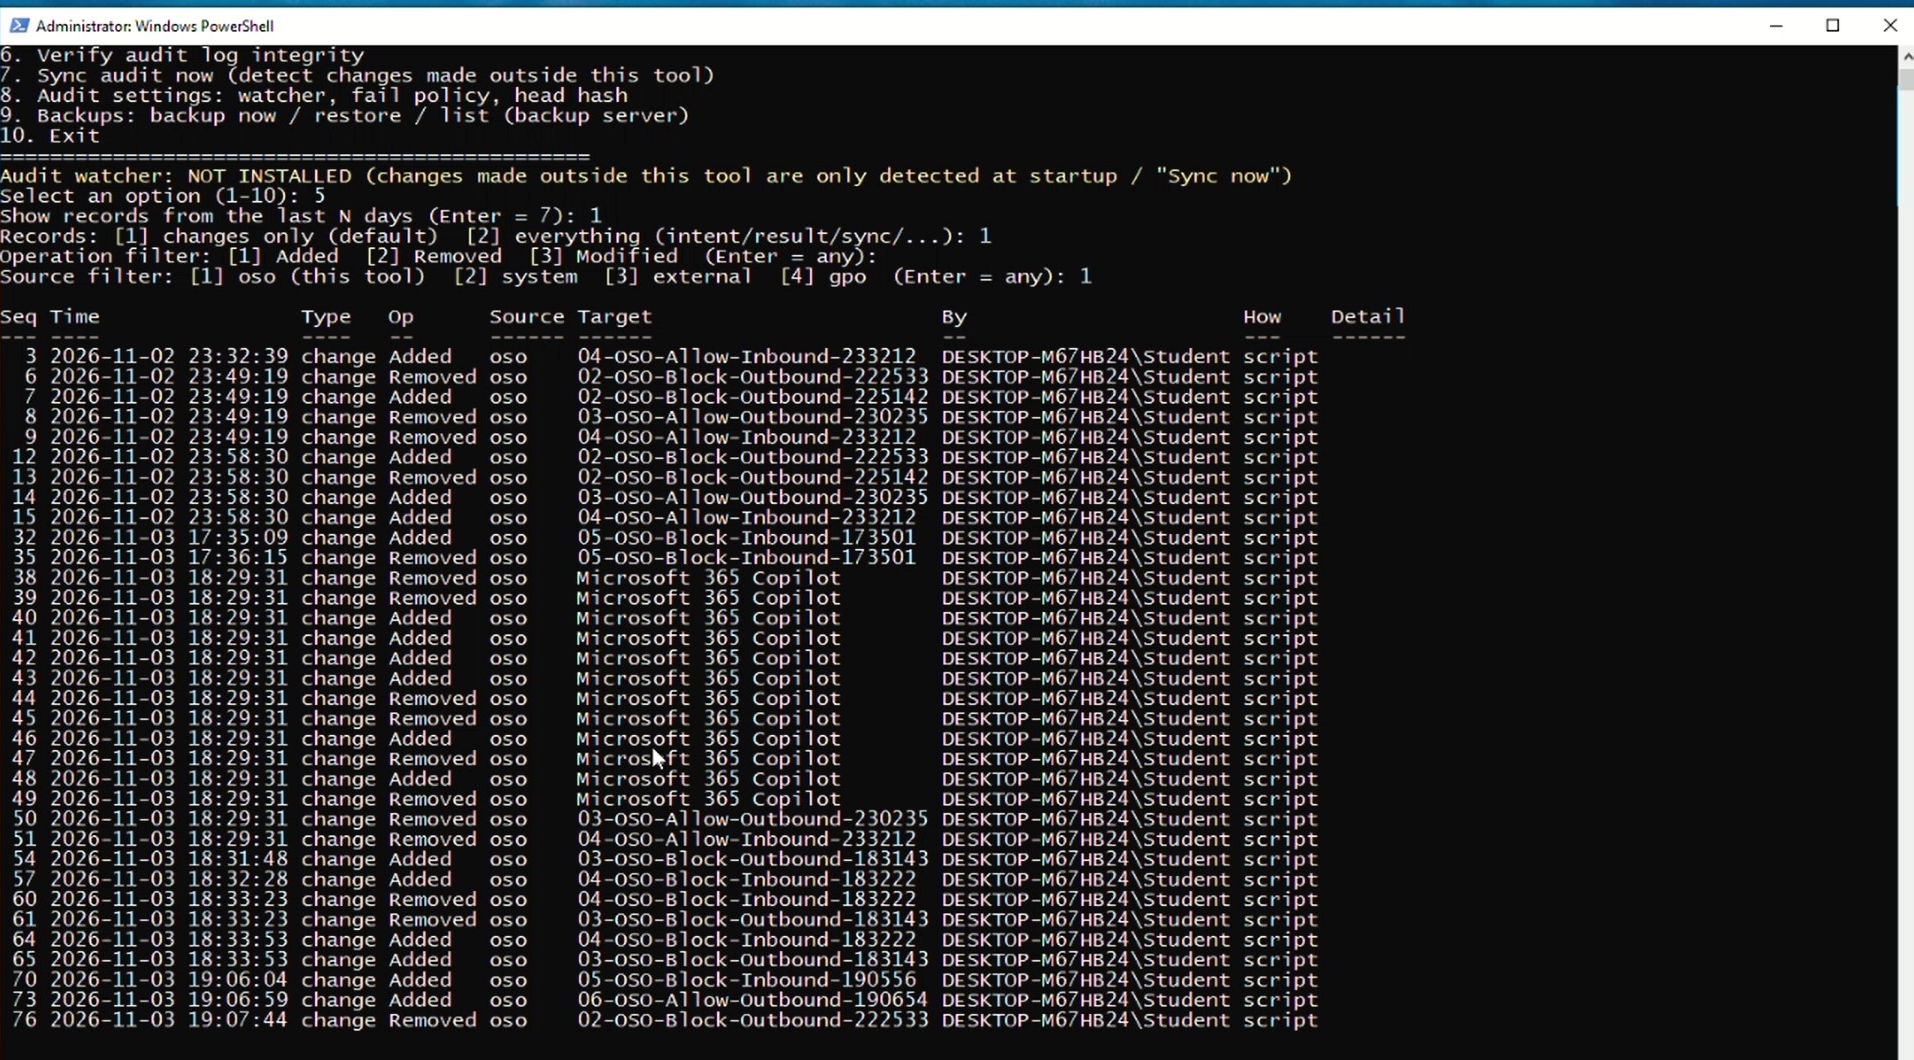
\includegraphics[width=\linewidth, keepaspectratio]{images/audit_log_view.png}
        \caption{Przeglądarka dziennika audytu (opcja menu 5) prezentująca chronologiczną historię zmian polityki wraz z identyfikacją użytkownika i metody detekcji}\label{fig:audit-log-sub1}
    \end{subfigure}\\[6pt]
    \begin{subfigure}[b]{\linewidth}
        \centering
        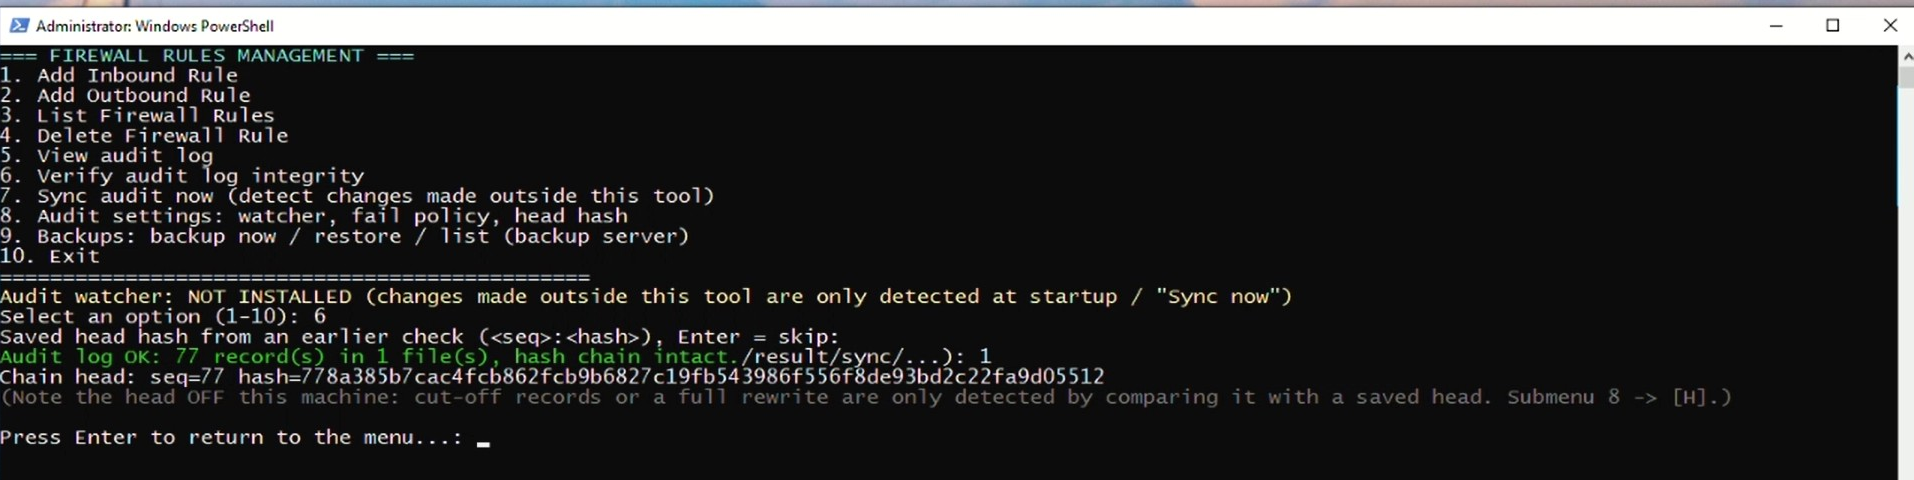
\includegraphics[width=\linewidth, keepaspectratio]{images/audit_integrity.png}
        \caption{Weryfikacja spójności kryptograficznego łańcucha skrótów SHA-256 dziennika audytu (opcja menu 6) wraz z wyznaczeniem bieżącego nagłówka (\textit{Chain head})}\label{fig:audit-integrity}
    \end{subfigure}
    \caption{Interaktywny podgląd historii zmian polityki oraz weryfikacja kryptograficznego łańcucha skrótów SHA-256 w Module 3}\label{fig:audit-log-view}
\end{figure}

\subsection{Wykrywanie zmian zewnętrznych (Watcher) i polityka fail-closed / fail-open}\label{subsec:watcher-i-failpolicy}

Modyfikacje polityki zapory wykonywane poza narzędziem (np.\ w graficznej przystawce \file{wf.msc}, poleceniem \cmd{netsh}, przez silnik zasad grupy GPO lub inny skrypt PowerShell) są przechwytywane przez usługę \textit{Watcher} instalowaną z poziomu podmenu opcji \code{8} (\code{[I] Install / update watcher}, rysunek \ref{fig:audit-watcher-install}). Podczas instalacji skrypt kopiuje sam siebie do izolowanego podkatalogu \file{C:\ProgramData\FirewallAudit\bin\firewall.ps1} zabezpieczonego listą ACL należącą do administratorów i rejestruje zadanie harmonogramu \code{\FirewallAudit\Watcher} uruchamiane na koncie \code{SYSTEM}.

Zadanie \textit{Watcher} jest wyzwalane przez trzy niezależne mechanizmy:
\begin{enumerate}
    \item \textbf{Wyzwalacz zdarzeniowy (\textit{Event Trigger})} - subskrypcja XPath na kanale dziennika zapory reagująca natychmiast na zdarzenia o identyfikatorach \code{2002}-\code{2006}, \code{2033}, \code{2052}, \code{2059} oraz \code{2097}-\code{2099}. Aby uniknąć wielokrotnego wyliczania migawek podczas masowych operacji (np.\ importu polityki generującego setki zdarzeń w ciągu kilku sekund), po uruchomieniu \textit{Watcher} odczekuje na ustabilizowanie licznika \code{RecordId} w dzienniku zdarzeń (brak nowych zdarzeń przez 3 kolejne sekundy, maksymalnie do 30 s), po czym wykonuje pojedynczą synchronizację zbiorczą.
    \item \textbf{Wyzwalacz startowy (\textit{AtStartup})} - weryfikacja stanu polityki podczas rozruchu systemu operacyjnego.
    \item \textbf{Wyzwalacz okresowy (co 15 minut)} - siatka bezpieczeństwa gwarantująca wykrycie zmian zewnętrznych nawet w sytuacji, gdy kanał dziennika zdarzeń zapory został wyłączony przez administratora, przepełniony lub wyczyszczony. Stan zdrowia zadania jest raportowany w pliku \file{state.json} i wyświetlany pod menu głównym (\code{Healthy}, \code{Failed}, \code{Stale} po braku udanego przebiegu przez $>45$ min).
\end{enumerate}

\Figure[1.0]{audit_watcher_install.png}{Podmenu ustawień audytu (opcja 8): diagnostyka dziennika zdarzeń zapory, konfiguracja polityki awarii oraz instalacja zadania systemowego \textit{Watcher}}{fig:audit-watcher-install}

Algorytm synchronizacji stanu polityki, korelacji zmian zewnętrznych z dziennikiem zdarzeń Windows oraz weryfikacji łańcucha skrótów przedstawiono w algorytmie \ref{alg:synchronizacja-i-weryfikacja}.

\begin{algorithm}[H]
    \caption{Synchronizacja stanu polityki zapory, atrybucja zmian zewnętrznych i weryfikacja łańcucha skrótów}\label{alg:synchronizacja-i-weryfikacja}
    \Input{Wyzwalacz $\mathit{Trig} \in \{\texttt{startup}, \texttt{manual}, \texttt{task}\}$, opcjonalny zapamiętany nagłówek łańcucha $\langle s_{\text{exp}}, h_{\text{exp}} \rangle$}
    \Output{Bilans wykrytych zmian zewnętrznych oraz raport integralności łańcucha dziennika}
    \textbf{Część A: Synchronizacja i wykrywanie zmian zewnętrznych (\code{Invoke-AuditSync})}\;
    Pozyskaj muteks \code{Global\FirewallAuditLog}, wczytaj bazę $B$, wykonaj migawkę $S_{\text{now}}$ i wylicz $\Delta \leftarrow \operatorname{CompareSnapshots}(B.\mathit{Entries}, S_{\text{now}})$\;
    Domknij przerwane transakcje (\code{intent} bez \code{result}) statusem \code{recovered} oraz uzgodnij znaczniki z \file{pending.jsonl} (\code{unlogged-change})\;
    \For{każdej różnicy $d \in \Delta$}{
        \lIf{klucz $d.\mathit{Key}$ należy do drzewa GPO}{$\mathit{src} \leftarrow \code{gpo}$; $\mathit{actor} \leftarrow \texttt{unknown (GPO engine)}$}
        \Else{
            Dopasuj zdarzenie z kanału \texttt{Firewall} po $\mathit{RuleId}$ i rozwiąż SID sprawcy $\operatorname{ResolveSid}(\mathit{ModifyingUser})$\;
            \lIf{SID systemowy \textbf{oraz} proces $\in \{\file{svchost.exe}, \file{services.exe}, \file{lsass.exe}\}$}{$\mathit{src} \leftarrow \code{system}$} \lElse{$\mathit{src} \leftarrow \code{external}$}
        }
        $\mathit{det} \leftarrow \text{jeżeli } \mathit{Trig} = \texttt{task} \text{ to } \code{watcher} \text{ w p.p. } \code{reconcile}$\;
        Zapisz rekord $\operatorname{WriteRecord}(\texttt{type}=\code{change}, d, \texttt{source}=\mathit{src}, \texttt{detection}=\mathit{det}, \texttt{actor}=\mathit{actor})$\;
    }
    \lIf{$\Delta \neq \emptyset$ \textbf{lub} odzyskano transakcje \textbf{lub} $\mathit{Trig} = \texttt{manual}$}{zapisz rekord \texttt{sync} z nowym skrótem $h_B$ i zaktualizuj \file{baseline.json}}
    Zwolnij muteks \code{Global\FirewallAuditLog}\;
    \textbf{Część B: Weryfikacja łańcucha skrótów (\code{Test-AuditLogIntegrity})}\;
    $h_{\text{prev}} \leftarrow 0^{64}$; $s_{\text{prev}} \leftarrow 0$; $\mathit{foundHead} \leftarrow \text{fałsz}$\;
    \For{każdego wiersza $L$ w plikach od najstarszego zrotowanego do \file{audit.jsonl}}{
        Wyodrębnij deklarowany skrót $h_{\text{claim}}$ oraz ciało rekordu $J \leftarrow L \setminus \{\code{hash}\}$\;
        \lIf{$\operatorname{SHA256}(J) \neq h_{\text{claim}}$ \textbf{lub} $J.\mathit{prev} \neq h_{\text{prev}}$ \textbf{lub} $J.\mathit{seq} \neq s_{\text{prev}} + 1$}{\textbf{zgłoś błąd} naruszenia ciągłości łańcucha}
        \If{podano $\langle s_{\text{exp}}, h_{\text{exp}} \rangle$ \textbf{oraz} $J.\mathit{seq} = s_{\text{exp}}$}{
            $\mathit{foundHead} \leftarrow \text{prawda}$; \lIf{$h_{\text{claim}} \neq h_{\text{exp}}$}{\textbf{zgłoś błąd} przepisania dziennika względem \textit{head hash}}
        }
        $h_{\text{prev}} \leftarrow h_{\text{claim}}$; $s_{\text{prev}} \leftarrow J.\mathit{seq}$\;
    }
    \lIf{podano $\langle s_{\text{exp}}, h_{\text{exp}} \rangle$ \textbf{oraz} $\mathit{foundHead} = \text{fałsz}$}{\textbf{zgłoś błąd} obcięcia końca dziennika}
    \Return{Raport spójności łańcucha oraz bilans synchronizacji}\;
\end{algorithm}

Moduł implementuje ponadto jawny mechanizm sterowania polityką reakcji na awarię dziennika (\textit{fail-closed} vs \textit{fail-open}):
\begin{itemize}
    \item \textbf{Tryb \code{Closed} (domyślny)} - nadrzędność rozliczalności: jeżeli dziennik audytu jest zablokowany przez inny proces po upływie czasu oczekiwania (60 s), uszkodzony lub katalog audytu ma nieprawidłowego właściciela, żadna zmiana polityki zapory nie zostaje wykonana.
    \item \textbf{Tryb \code{Open} (awaryjny)} - umożliwia wykonanie zmiany w sytuacji awarii dziennika, jednak zmiana trybu na \code{Open} wymaga podania powodu i zapisania wyprzedzającego rekordu \code{setting} w samym dzienniku audytu wraz ze skrótem pliku \file{settings.json}. Ręczna edycja pliku \file{settings.json} w notatniku w celu cichego wyłączenia blokady jest wykrywana przy starcie (skrót w pliku nie zgadza się z ostatnim rekordem \code{setting} w dzienniku), co automatycznie wymusza powrót do trybu \code{Closed} i rejestruje incydent \code{settings-file-modified}. Ponadto aktywny tryb \code{Open} wyświetla w menu głównym czerwony baner ostrzegawczy \code{AUDIT FAIL-OPEN}, a każda wykonana w tym czasie zmiana odkłada znacznik w pliku \file{pending.jsonl} (lub w systemowym dzienniku zdarzeń \code{Application} o ID \code{4001}).
\end{itemize}

\section{Moduł 4: Zdalne kopie zapasowe i odtwarzanie polityki}\label{sec:modul-backup}

Czwarty moduł funkcjonalny (autor: Ruslan Hedz) odpowiada za automatyczne oraz ręczne tworzenie kopii zapasowych pełnej polityki zapory na zewnętrznym serwerze Ubuntu (\code{10.0.2.30}), ich inwentaryzację oraz bezpieczne przywracanie na stacji roboczej Windows (\code{10.0.2.20}).

\subsection{Architektura komunikacji klient-serwer i protokół eksportu (pull)}\label{subsec:eksport-konfiguracji}

Aby uniemożliwić stacji klienckiej nadpisywanie lub kasowanie historycznych kopii zapasowych na serwerze, proces tworzenia kopii realizowany jest w architekturze odwróconego pobierania (\textit{server-side pull}):

\begin{enumerate}
    \item \textbf{Inicjacja kopii przez klienta} - stacja Windows (automatycznie przed modyfikacją reguł lub ręcznie w podmenu kopii) nawiązuje połączenie SSH z kontem \code{fwbackup@10.0.2.30} na porcie 22, przekazując polecenie \textbf{backup <powód>} (ze zdefiniowaną listą dopuszczalnych powodów: \code{manual}, \code{auto-add}, \code{auto-delete}, \code{pre-restore} lub \code{scheduled}).
    \item \textbf{Weryfikacja i blokada na serwerze} - demon \code{sshd} na serwerze Ubuntu ignoruje oryginalne polecenie powłoki i na podstawie dyrektywy wymuszonego polecenia (\code{command=...}) w pliku \file{authorized_keys} uruchamia skrypt \file{fw-server.sh} ze sztywno przypisaną tożsamością klienta. Skrypt sprawdza klienta w pliku \file{/etc/fwbackup/clients.conf} (nie ufając argumentom) i zakłada blokadę \cmd{flock}.
    \item \textbf{Pobranie polityki przez serwer (Agent Export)} - serwer Ubuntu nawiązuje połączenie zwrotne SSH na port 22 stacji Windows przy użyciu klucza prywatnego \file{/etc/fwbackup/id_export} (do 3 prób). Na stacji Windows klucz ten w pliku \file{administrators_authorized_keys} ma zablokowane powłoki i tunele (\code{restrict}) i wymusza uruchomienie wyłącznie agenta eksportu:
    \begin{center}
        \code{powershell.exe -NoProfile -ExecutionPolicy Bypass -File C:/FW/FirewallRules.ps1 -Agent Export}
    \end{center}
    Agent eksportuje politykę poleceniem \cmd{netsh.exe advfirewall export} do chronionego katalogu tymczasowego, oblicza skrót SHA-256 i zwraca przez strumień \code{stdout} ustrukturyzowaną odpowiedź: nagłówek \code{FWAGENT-BEGIN}, pola \code{COMPUTER=<nazwa>}, \code{SHA256=<hash>}, \code{SIZE=<bajty>}, blok \code{DATA} z zawartością pliku \file{.wfw} zakodowaną w Base64 oraz stopkę \code{FWAGENT-END}.
    \item \textbf{Weryfikacja i zapis na serwerze} - skrypt \file{fw-server.sh} dekoduje strumień Base64, oblicza niezależnie skrót SHA-256 odebranego pliku binarnego i porównuje go z wartością zadeklarowaną przez agenta. W przypadku zgodności zapisuje kopię w katalogu \file{/srv/fwbackups/<user>/backups/} pod nazwą:
    \[
        \texttt{<KOMPUTER>\_<YYYYMMDD>\_<HHMMSS>\_<powód>.wfw}
    \]
    oraz bliźniaczy plik sumy kontrolnej \file{.wfw.sha256}. Zapis wykonywany jest do plików tymczasowych \file{.part} z zamianą (\cmd{mv -f}) oraz dziedziczeniem grupy \code{sftpgo} (bit \code{setgid} \code{2750} na katalogu), przy czym plik \file{.sha256} tworzony jest jako ostatni - dzięki temu klient listujący katalog przez SFTP widzi wyłącznie kompletne, zweryfikowane kopie. Na końcu serwer wykonuje retencję (\code{prune}), zachowując 30 najnowszych kopii automatycznych (\code{auto-*} oraz \code{scheduled}), nigdy nie usuwając kopii manualnych ani kopii aktualnie odtwarzanej.
\end{enumerate}

\subsection{Dwufazowa procedura odtwarzania polityki (Restore) i weryfikacja spójności}\label{subsec:import-konfiguracji}

Odtwarzanie polityki zapory (opcja menu \code{9} $\rightarrow$ \code{[R]}) zostało zaprojektowane tak, aby serwer kopii nie posiadał uprawnień do zdalnego wgrywania polityki na stację Windows (eliminuje to ryzyko przejęcia stacji roboczych w przypadku kompromitacji serwera kopii oraz rozwiązuje problem blokowania potoków wejściowych SSH):

\begin{enumerate}
    \item \textbf{Inwentaryzacja i wybór kopii} - klient łączy się przez protokół SFTP z serwerem SFTPGo na porcie 2022, pobiera listę plików z wirtualnego katalogu \file{backups/}, filtruje wyłącznie wpisy posiadające parę \file{.wfw} + \file{.wfw.sha256} i wyświetla tabelę zawierającą indeks, datę, powód utworzenia oraz nazwę pliku (rysunek \ref{fig:backup-restore}).
    \item \textbf{Faza I (Przygotowanie na serwerze i kopia ratunkowa \code{pre-restore})} - po wybraniu numeru kopii, podaniu decyzji o utworzeniu kopii ratunkowej bieżącego stanu (domyślnie \code{yes}) oraz wpisaniu słowa potwierdzającego \code{RESTORE}, klient wysyła do serwera po SSH rozkaz \code{restore <plik.wfw> <yes|no>}. Serwer oznacza wskazaną kopię jako chronioną przed retencją (\code{PROTECT}), sprawdza jej integralność SHA-256 na dysku serwera, wykonuje kopię ratunkową bieżącej polityki z powodem \code{pre-restore}, ponownie weryfikuje plik docelowy i zwraca potwierdzenie \code{STATUS=OK}.
    \item \textbf{Faza II (Pobranie po SFTP, weryfikacja lokalna i zaudytowany import)} - po otrzymaniu potwierdzenia z serwera stacja Windows pobiera plik \file{<plik>.wfw} oraz \file{<plik>.wfw.sha256} przez SFTPGo (korzystając z uprawnień tylko do odczytu \code{list} + \code{download}), wylicza lokalnie skrót SHA-256 pobranego pliku i porównuje go ze skrótem z pliku \file{.sha256}. Dopiero po pozytywnej weryfikacji kryptograficznej wywoływany jest transakcyjny mechanizm audytu (\code{Operation = 'Restore'}, \code{Scope = 'All'}), wewnątrz którego wykonywany jest import \cmd{netsh.exe advfirewall import} oraz natychmiastowe wywołanie procedury \code{EnsureSshRule()}. Ponieważ odtwarzanie jest inicjowane bezpośrednio z lokalnej konsoli administratora, import starszej polityki pozbawionej reguły \code{FWBackup-SSH-In} nie przerywa sesji konsolowej, a reguła dostępowa dla serwera kopii zostaje odtworzona zanim system obsłuży jakiekolwiek nowe pakiety sieciowe.
\end{enumerate}

Przebieg procedury wyboru kopii, wykonania zrzutu ratunkowego \code{pre-restore} i przywrócenia polityki oraz zaktualizowaną listę kopii na serwerze przedstawiono na rysunku \ref{fig:backup-restore}.

\begin{figure}[H]
    \centering
    \begin{subfigure}[b]{\linewidth}
        \centering
        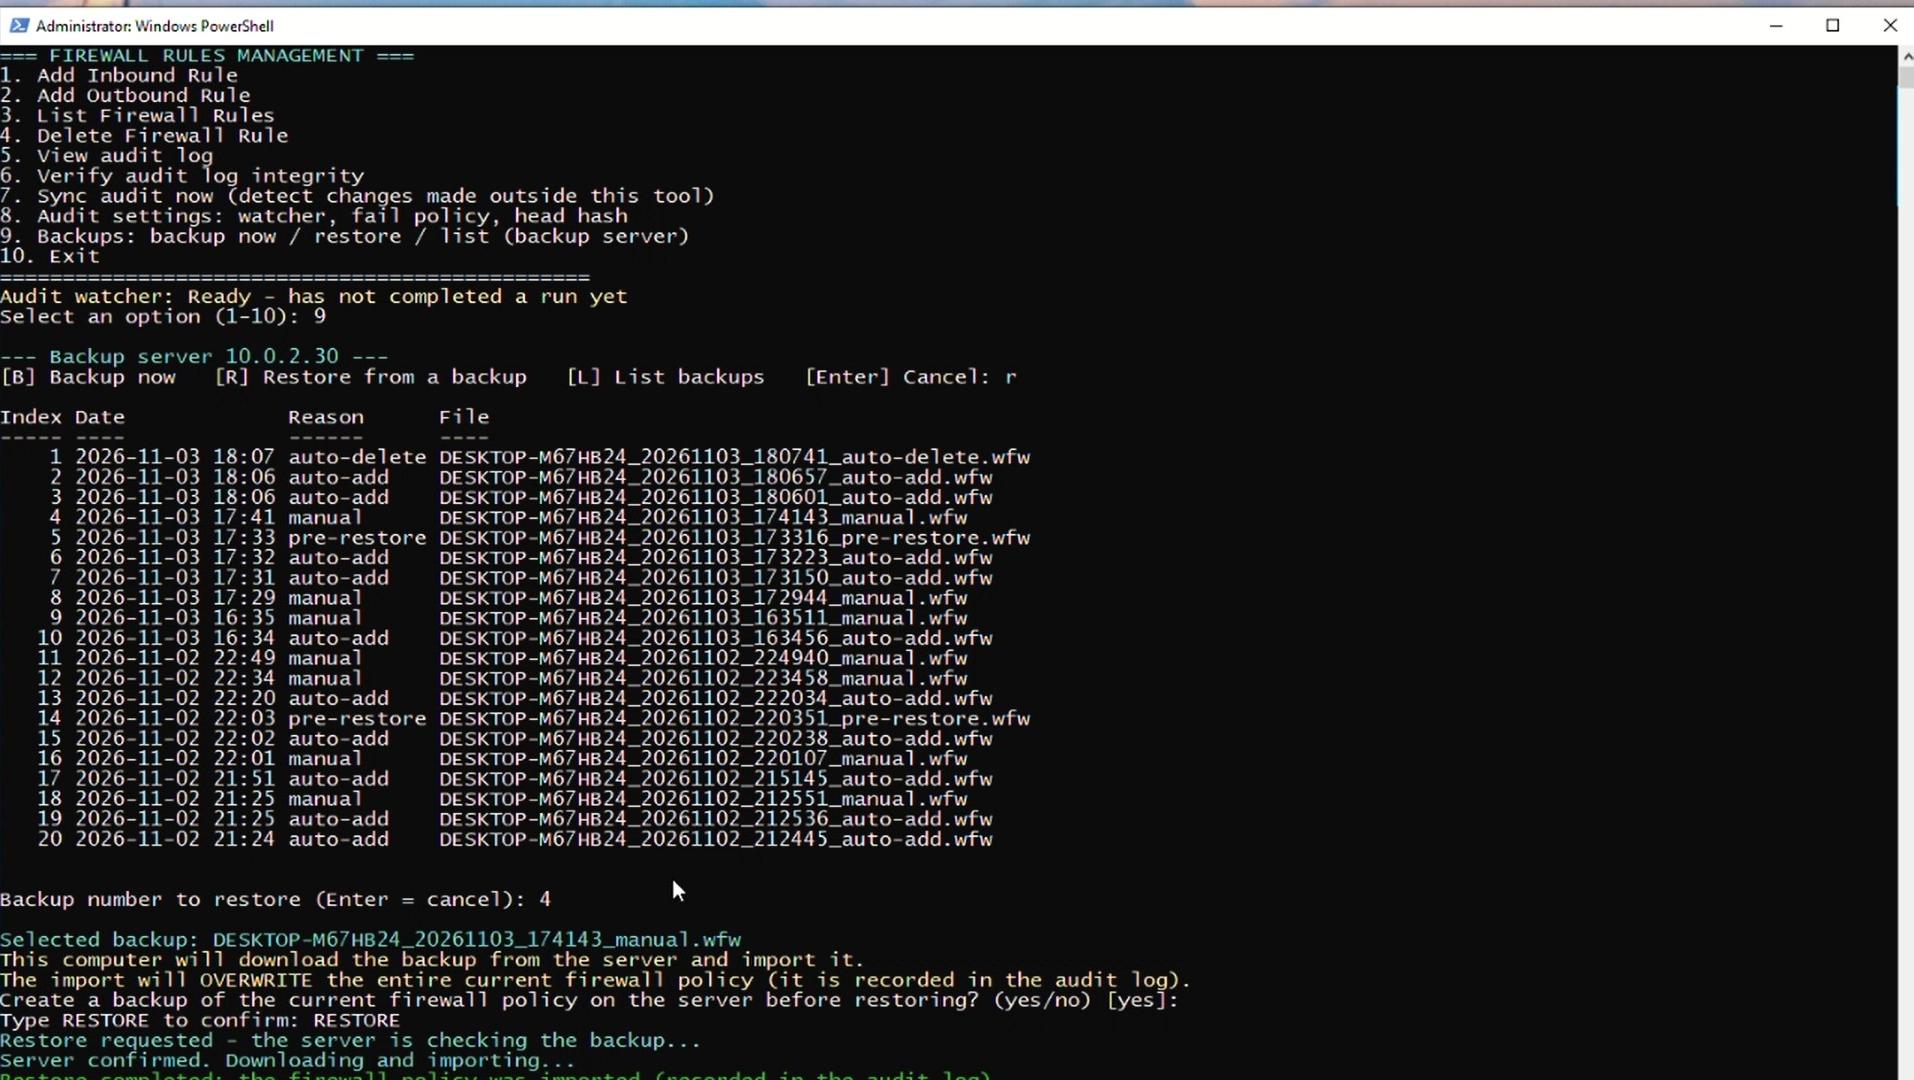
\includegraphics[width=\linewidth, keepaspectratio]{images/backup_restore.png}
        \caption{Procedura przywracania polityki zapory (opcja menu 9 $\rightarrow$ R) z utworzeniem kopii ratunkowej \code{pre-restore} i potwierdzeniem \code{RESTORE}}\label{fig:backup-restore-sub1}
    \end{subfigure}\\[6pt]
    \begin{subfigure}[b]{\linewidth}
        \centering
        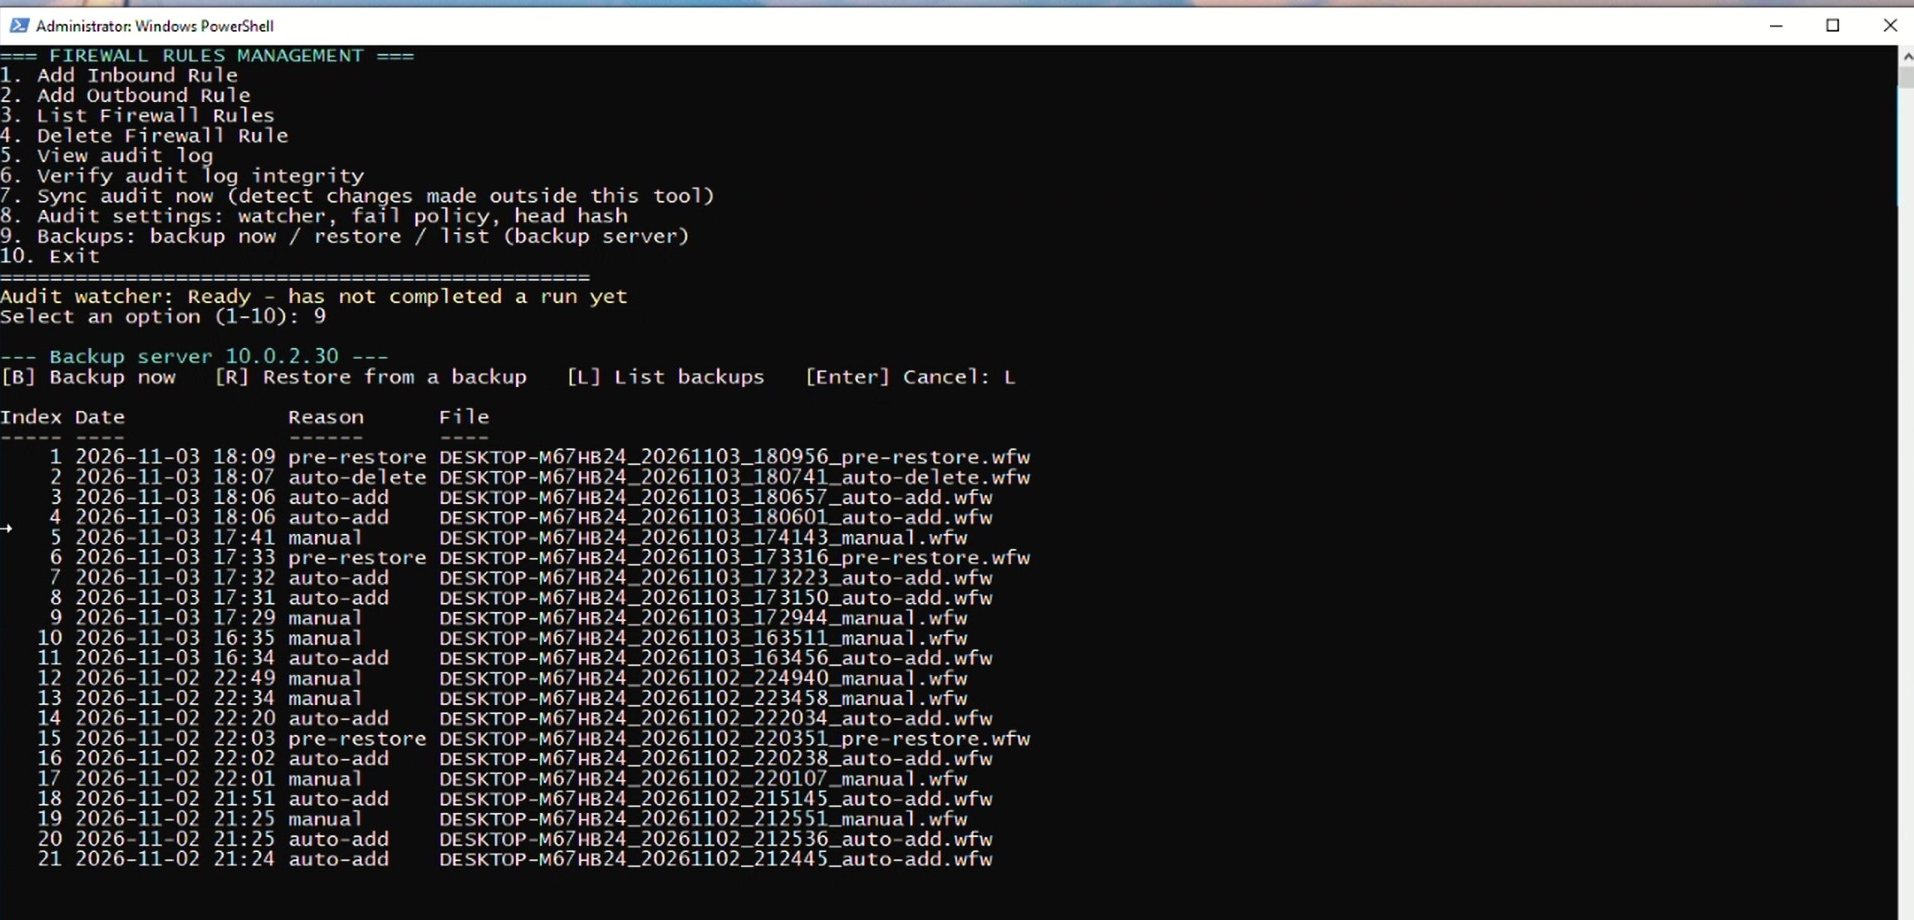
\includegraphics[width=\linewidth, keepaspectratio]{images/backup_list.png}
        \caption{Lista kopii zapasowych na serwerze \code{10.0.2.30} po zakończeniu odtwarzania, uwzględniająca nowo utworzoną kopię \code{pre-restore}}\label{fig:backup-list}
    \end{subfigure}
    \caption{Dwufazowe odtwarzanie polityki zapory z serwera zdalnego oraz inwentaryzacja kopii przez kanał SFTPGo w Module 4}\label{fig:backup-restore}
\end{figure}

Formalny zapis algorytmu tworzenia kopii w modelu \textit{pull} oraz dwufazowego odtwarzania konfiguracji przedstawiono w algorytmie \ref{alg:backup-i-restore}.

\begin{algorithm}[H]
    \caption{Zdalne tworzenie kopii zapasowej w modelu \textit{pull} oraz dwufazowe odtwarzanie polityki zapory}\label{alg:backup-i-restore}
    \Input{Tryb $M \in \{\texttt{Backup}, \texttt{Restore}\}$, powód $\mathit{Reason}$ lub plik kopii $F_{\text{target}}$ i flaga $\mathit{Pre} \in \{\texttt{yes}, \texttt{no}\}$}
    \Output{Status operacji kopii zapasowej lub zaudytowanego odtworzenia polityki zapory}
    \If{$M = \texttt{Backup}$}{
        Klient wysyła po SSH (port 22, wymuszone polecenie) żądanie $\code{backup } \parallel \mathit{Reason}$; serwer zakłada blokadę \cmd{flock}\;
        Serwer łączy się zwrotnie po SSH (klucz \file{id_export}) ze stacją Windows, wywołując \code{-Agent Export}\;
        Agent weryfikuje regułę \texttt{FWBackup-SSH-In}, wykonuje \cmd{netsh advfirewall export} do pliku $T$, wylicza $h_{\text{win}} \leftarrow \operatorname{SHA256}(T)$ i zwraca $\operatorname{Base64}(T)$\;
        Serwer dekoduje strumień do pliku $T_{\text{srv}}$ i wylicza $h_{\text{srv}} \leftarrow \operatorname{SHA256}(T_{\text{srv}})$\;
        \lIf{$T_{\text{srv}}$ jest pusty \textbf{lub} $h_{\text{srv}} \neq h_{\text{win}}$}{\Return{\texttt{FAIL: niezgodność sumy kontrolnej SHA-256 lub błąd eksportu}}}
        Zapisz atomowo $\mathit{Name}.\file{wfw}$ oraz $\mathit{Name}.\file{wfw.sha256}$ (grupa \texttt{sftpgo}, prawa \texttt{0640}) i usuń nadmiarowe kopie ponad $\mathit{KEEP\_AUTO} = 30$\;
        \Return{$\texttt{OK: } \mathit{Name}.\file{wfw}$}\;
    }
    \ElseIf{$M = \texttt{Restore}$}{
        Klient pobiera przez SFTPGo (port 2022) listę par $\file{*.wfw} + \file{*.wfw.sha256}$; po wpisaniu \texttt{RESTORE} wysyła po SSH $\code{restore } \parallel F_{\text{target}} \parallel \text{\code{ }} \parallel \mathit{Pre}$\;
        Serwer oznacza $F_{\text{target}}$ jako chroniony ($\mathit{PROTECT}$) i weryfikuje jego skrót SHA-256 na dysku\;
        \If{$\mathit{Pre} = \texttt{yes}$}{
            Serwer wykonuje kopię ratunkową z powodem $\code{pre-restore}$; \lIf{błąd kopii}{\Return{\texttt{FAIL: przerwano przed nadpisaniem polityki}}}
        }
        Klient pobiera przez SFTPGo pliki $F_{\text{target}}$ i $F_{\text{target}}.\file{sha256}$, wylicza lokalnie $h_{\text{calc}} \leftarrow \operatorname{SHA256}(F_{\text{target}})$ i porównuje z $h_{\text{exp}}$\;
        \lIf{$h_{\text{calc}} \neq h_{\text{exp}}$}{usuń pliki tymczasowe i \textbf{zgłoś wyjątek} \enquote{Niezgodność SHA-256 pobranej kopii - import zablokowany}}
        Wykonaj $\operatorname{AuditedChange}\bigl(\texttt{Operation}=\code{Restore},\; \texttt{Scope}=\texttt{All},\; \texttt{Action}=\{\cmd{netsh advfirewall import } F_{\text{target}};\; \operatorname{EnsureSshRule}()\}\bigr)$\;
        Usuń pliki tymczasowe i \Return{\texttt{OK: polityka przywrócona i zarejestrowana w audycie}}\;
    }
\end{algorithm}
